\chapter{前言}

本研究旨在尋找具有最大面積的\emph{交圓內接三角形}。
「交圓內接三角形」一詞最早由楊家婕 \cite{yang} 提出,
而後我在〈再探交圓內接三角形:極大三角形的構造〉\cite{liu} 中給出了更嚴謹的定義。
我將其重述如下:

\begin{definition}[交圓內接三角形]
給定兩相交圓。
考慮它們各自圍成的兩個圓盤的交集。
內接於其邊界的三角形即稱作這對圓的\emph{交圓內接三角形} (如圖 \ref{fig:triangleincircles})。
\begin{figure}
\centering
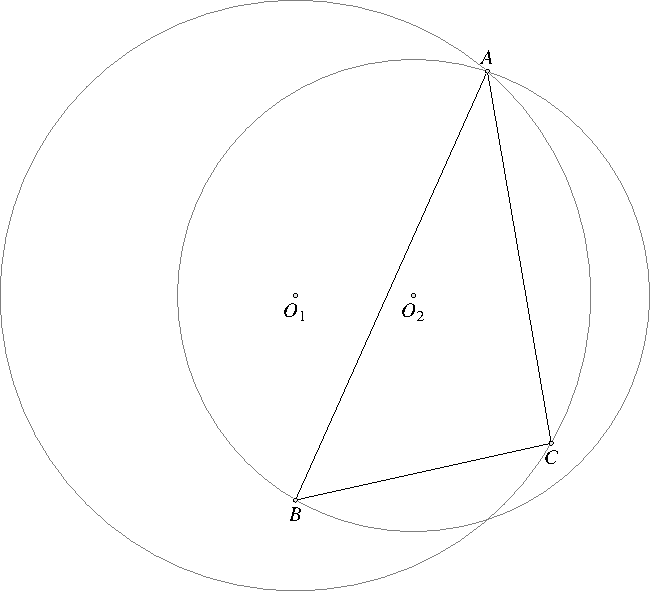
\includegraphics{graphics/triangleincircles}
\caption{交圓內接三角形:圖中的 $\triangle ABC$ 是圓 $O_1$ 和圓 $O_2$ 的一個交圓內接三角形。}
\label{fig:triangleincircles}
\end{figure}
\end{definition}


關於此問題已有不少的研究報告 \cite{chen, chien, yang, liu}。
這些報告分別在不同的競賽取得不同的獎項,
但沒有任何一人真正完全解決此問題——
而本研究將對此提出完整的解答。
